\documentclass[12pt, a4paper]{report}
\usepackage[utf8]{inputenc}
\usepackage[T1]{fontenc}
\usepackage[utf8]{inputenc}
\usepackage{geometry}
\usepackage{listings}
\usepackage{xcolor}
\usepackage[]{graphicx}
\usepackage[export]{adjustbox}
\usepackage{subcaption}
\makeatletter
\setlength{\@fptop}{0pt}
\makeatother

\definecolor{codegreen}{rgb}{0.26, 0.61, 0}
\definecolor{codegray}{rgb}{0.5,0.5,5}
\definecolor{codepurple}{rgb}{58,0,0.82}
\definecolor{backcolour}{rgb}{0.80, 0.81, 0.93}

\lstdefinestyle{mystyle}{
    backgroundcolor=\color{backcolour},   
    commentstyle=\color{codegreen},
    keywordstyle=\color{magenta},
    numberstyle=\tiny\color{codegray},
    stringstyle=\color{codepurple},
    basicstyle=\ttfamily\footnotesize,
    breakatwhitespace=false,         
    breaklines=true,                 
    captionpos=b,                    
    keepspaces=true,                 
    numbers=left,                    
    numbersep=5pt,                  
    showspaces=false,                
    showstringspaces=false,
    showtabs=false,                  
    tabsize=2
}

\lstset{style=mystyle}


\title{\textbf{EE2703: Applied Programming Lab\\Assignment 6A\\Tubelight Simulation
}}


\author{Devaganthan S S\\ EE19B018}
\date{\today}
\begin{document}

\maketitle


\section{Abstract}
This assignment aims to Understand how Simulations can be Done in Python


\section{Introduction}
We try to simulate a 1-Dimensional Model of a Tubelight. A uniform Electric Field exists across the length of the Tubelight. Electrons are Injected at the cathode end of the tube light, which initially has zero energy. Due to the Electric Field, the electrons gain Kinetic Energy. When the Electrons gain a Threshold Energy, say E0, upon collision with Atoms in the Tube lights, the energy of the Electron is completely transferred to the atom which excites the atom, resulting in Light Emission. The Uncollided Electrons hit the other end of the tube light and loose all the energy. We try to simulate the Tube Light in Python. We plot the Light Intensity vs Position, Electron Density Vs Position, Phase space Diagram.
\section{Results and Implementation}
\subsection{Initialization}
We initialize the parameters that define the Tube Light Model. The parameters can also be given via the Command Line Arguments. The below code initializes the parameters
\noindent
\lstinputlisting[language = python]{code1.py}
\subsection{Iteration}
We execute a for loop $nk$ number of times. In each iteration, we record positions of un-collided electrons, corresponding Velocities, the Displacement it had traveled as a array. From these vectors, we find the Intensity of Light, Electron Density, Velocity of Electron at each position over the $nk$ Iterations. The below code executes the $"For"$ Loop.

\lstinputlisting[language = python]{code2.py}

\subsection{Histogram for Light Intensity}
We plot a Histogram Graph for the Light intensity vs Position, with the list “I” obtained from the For Loop. We can see that the Light Intensity is almost constant in the middle, from the Plot. The Below code plots the Histogram. The Program also outputs the Intensity in a tabular form
\noindent
\lstinputlisting[language = python]{code3.py}
\begin{figure}[h!]
    \centering
    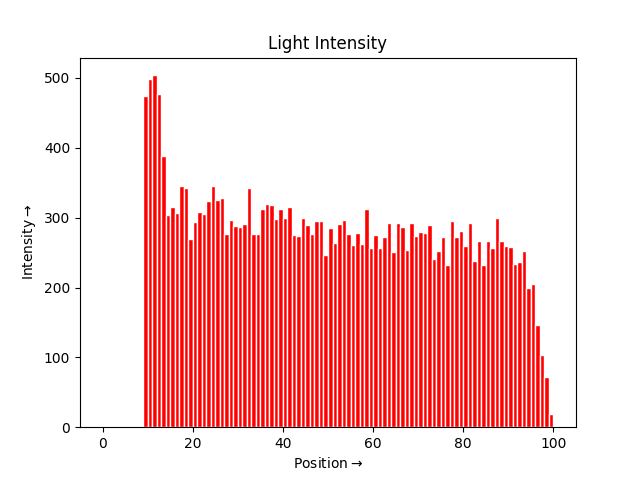
\includegraphics[scale=0.5125]{fig1.png} 
    \caption{}
    \label{fig:my_label}
\end{figure}
\subsection{Histogram for Electron Density}
We plot a Histogram Graph for the Electron Density vs Position, with the list “X” obtained from the For Loop. We can see that the Electron Density is almost constant in the middle, from the Plot. There is also a peak at the start since electrons are injected at n=0  The Below code plots the Histogram. 
\noindent
\lstinputlisting[language = python]{code4.py}
\begin{figure}[h!]
    \centering
    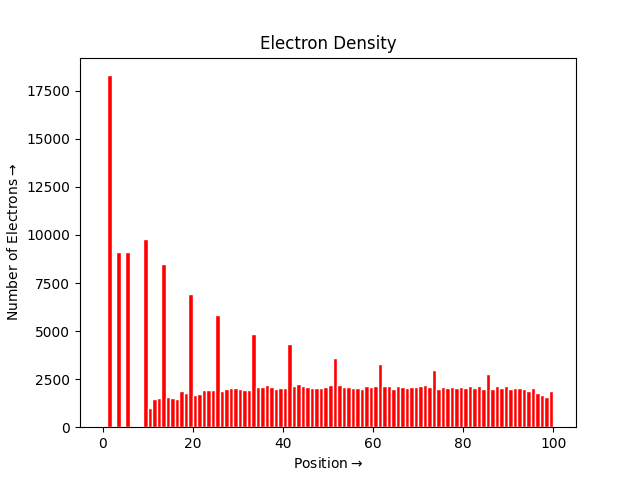
\includegraphics[scale=0.6]{fig2.png} 
    \caption{}
    \label{fig:my_label}
\end{figure}
\subsection{Phase Space Diagram}
For each Electron, we plot its corresponding position and Velocity to get the Phase space diagram. From the Plot we can see that the electron velocity increases as "n" increases, but the electron Density decreases. The below plots the phase space.
\noindent
\lstinputlisting[language = python]{code5.py}
\begin{figure}[h!]
    \centering
    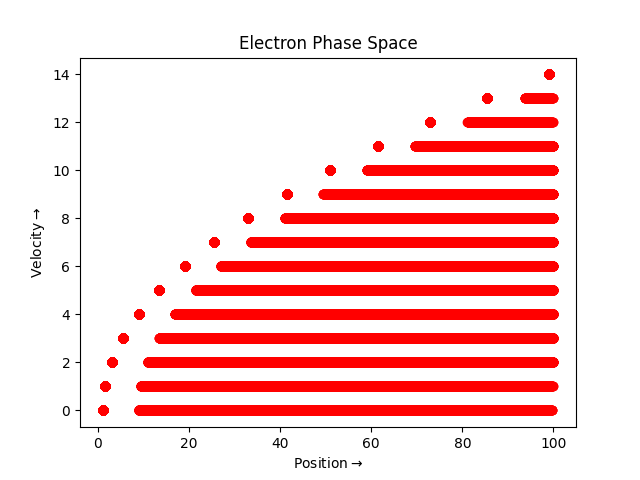
\includegraphics[scale=0.6]{fig3.png} 
    \caption{}
    \label{fig:my_label}
\end{figure}

\section{Conclusion}
The Tube Light Model was simulated using Python. We learnt how to Plot Population Plots in Python.


\end{document}

